% Options for packages loaded elsewhere
\PassOptionsToPackage{unicode}{hyperref}
\PassOptionsToPackage{hyphens}{url}
\PassOptionsToPackage{dvipsnames,svgnames,x11names}{xcolor}
%
\documentclass[
  letterpaper,
  DIV=11,
  numbers=noendperiod]{scrartcl}

\usepackage{amsmath,amssymb}
\usepackage{iftex}
\ifPDFTeX
  \usepackage[T1]{fontenc}
  \usepackage[utf8]{inputenc}
  \usepackage{textcomp} % provide euro and other symbols
\else % if luatex or xetex
  \usepackage{unicode-math}
  \defaultfontfeatures{Scale=MatchLowercase}
  \defaultfontfeatures[\rmfamily]{Ligatures=TeX,Scale=1}
\fi
\usepackage{lmodern}
\ifPDFTeX\else  
    % xetex/luatex font selection
\fi
% Use upquote if available, for straight quotes in verbatim environments
\IfFileExists{upquote.sty}{\usepackage{upquote}}{}
\IfFileExists{microtype.sty}{% use microtype if available
  \usepackage[]{microtype}
  \UseMicrotypeSet[protrusion]{basicmath} % disable protrusion for tt fonts
}{}
\makeatletter
\@ifundefined{KOMAClassName}{% if non-KOMA class
  \IfFileExists{parskip.sty}{%
    \usepackage{parskip}
  }{% else
    \setlength{\parindent}{0pt}
    \setlength{\parskip}{6pt plus 2pt minus 1pt}}
}{% if KOMA class
  \KOMAoptions{parskip=half}}
\makeatother
\usepackage{xcolor}
\setlength{\emergencystretch}{3em} % prevent overfull lines
\setcounter{secnumdepth}{-\maxdimen} % remove section numbering
% Make \paragraph and \subparagraph free-standing
\ifx\paragraph\undefined\else
  \let\oldparagraph\paragraph
  \renewcommand{\paragraph}[1]{\oldparagraph{#1}\mbox{}}
\fi
\ifx\subparagraph\undefined\else
  \let\oldsubparagraph\subparagraph
  \renewcommand{\subparagraph}[1]{\oldsubparagraph{#1}\mbox{}}
\fi

\usepackage{color}
\usepackage{fancyvrb}
\newcommand{\VerbBar}{|}
\newcommand{\VERB}{\Verb[commandchars=\\\{\}]}
\DefineVerbatimEnvironment{Highlighting}{Verbatim}{commandchars=\\\{\}}
% Add ',fontsize=\small' for more characters per line
\usepackage{framed}
\definecolor{shadecolor}{RGB}{241,243,245}
\newenvironment{Shaded}{\begin{snugshade}}{\end{snugshade}}
\newcommand{\AlertTok}[1]{\textcolor[rgb]{0.68,0.00,0.00}{#1}}
\newcommand{\AnnotationTok}[1]{\textcolor[rgb]{0.37,0.37,0.37}{#1}}
\newcommand{\AttributeTok}[1]{\textcolor[rgb]{0.40,0.45,0.13}{#1}}
\newcommand{\BaseNTok}[1]{\textcolor[rgb]{0.68,0.00,0.00}{#1}}
\newcommand{\BuiltInTok}[1]{\textcolor[rgb]{0.00,0.23,0.31}{#1}}
\newcommand{\CharTok}[1]{\textcolor[rgb]{0.13,0.47,0.30}{#1}}
\newcommand{\CommentTok}[1]{\textcolor[rgb]{0.37,0.37,0.37}{#1}}
\newcommand{\CommentVarTok}[1]{\textcolor[rgb]{0.37,0.37,0.37}{\textit{#1}}}
\newcommand{\ConstantTok}[1]{\textcolor[rgb]{0.56,0.35,0.01}{#1}}
\newcommand{\ControlFlowTok}[1]{\textcolor[rgb]{0.00,0.23,0.31}{#1}}
\newcommand{\DataTypeTok}[1]{\textcolor[rgb]{0.68,0.00,0.00}{#1}}
\newcommand{\DecValTok}[1]{\textcolor[rgb]{0.68,0.00,0.00}{#1}}
\newcommand{\DocumentationTok}[1]{\textcolor[rgb]{0.37,0.37,0.37}{\textit{#1}}}
\newcommand{\ErrorTok}[1]{\textcolor[rgb]{0.68,0.00,0.00}{#1}}
\newcommand{\ExtensionTok}[1]{\textcolor[rgb]{0.00,0.23,0.31}{#1}}
\newcommand{\FloatTok}[1]{\textcolor[rgb]{0.68,0.00,0.00}{#1}}
\newcommand{\FunctionTok}[1]{\textcolor[rgb]{0.28,0.35,0.67}{#1}}
\newcommand{\ImportTok}[1]{\textcolor[rgb]{0.00,0.46,0.62}{#1}}
\newcommand{\InformationTok}[1]{\textcolor[rgb]{0.37,0.37,0.37}{#1}}
\newcommand{\KeywordTok}[1]{\textcolor[rgb]{0.00,0.23,0.31}{#1}}
\newcommand{\NormalTok}[1]{\textcolor[rgb]{0.00,0.23,0.31}{#1}}
\newcommand{\OperatorTok}[1]{\textcolor[rgb]{0.37,0.37,0.37}{#1}}
\newcommand{\OtherTok}[1]{\textcolor[rgb]{0.00,0.23,0.31}{#1}}
\newcommand{\PreprocessorTok}[1]{\textcolor[rgb]{0.68,0.00,0.00}{#1}}
\newcommand{\RegionMarkerTok}[1]{\textcolor[rgb]{0.00,0.23,0.31}{#1}}
\newcommand{\SpecialCharTok}[1]{\textcolor[rgb]{0.37,0.37,0.37}{#1}}
\newcommand{\SpecialStringTok}[1]{\textcolor[rgb]{0.13,0.47,0.30}{#1}}
\newcommand{\StringTok}[1]{\textcolor[rgb]{0.13,0.47,0.30}{#1}}
\newcommand{\VariableTok}[1]{\textcolor[rgb]{0.07,0.07,0.07}{#1}}
\newcommand{\VerbatimStringTok}[1]{\textcolor[rgb]{0.13,0.47,0.30}{#1}}
\newcommand{\WarningTok}[1]{\textcolor[rgb]{0.37,0.37,0.37}{\textit{#1}}}

\providecommand{\tightlist}{%
  \setlength{\itemsep}{0pt}\setlength{\parskip}{0pt}}\usepackage{longtable,booktabs,array}
\usepackage{calc} % for calculating minipage widths
% Correct order of tables after \paragraph or \subparagraph
\usepackage{etoolbox}
\makeatletter
\patchcmd\longtable{\par}{\if@noskipsec\mbox{}\fi\par}{}{}
\makeatother
% Allow footnotes in longtable head/foot
\IfFileExists{footnotehyper.sty}{\usepackage{footnotehyper}}{\usepackage{footnote}}
\makesavenoteenv{longtable}
\usepackage{graphicx}
\makeatletter
\def\maxwidth{\ifdim\Gin@nat@width>\linewidth\linewidth\else\Gin@nat@width\fi}
\def\maxheight{\ifdim\Gin@nat@height>\textheight\textheight\else\Gin@nat@height\fi}
\makeatother
% Scale images if necessary, so that they will not overflow the page
% margins by default, and it is still possible to overwrite the defaults
% using explicit options in \includegraphics[width, height, ...]{}
\setkeys{Gin}{width=\maxwidth,height=\maxheight,keepaspectratio}
% Set default figure placement to htbp
\makeatletter
\def\fps@figure{htbp}
\makeatother
% definitions for citeproc citations
\NewDocumentCommand\citeproctext{}{}
\NewDocumentCommand\citeproc{mm}{%
  \begingroup\def\citeproctext{#2}\cite{#1}\endgroup}
\makeatletter
 % allow citations to break across lines
 \let\@cite@ofmt\@firstofone
 % avoid brackets around text for \cite:
 \def\@biblabel#1{}
 \def\@cite#1#2{{#1\if@tempswa , #2\fi}}
\makeatother
\newlength{\cslhangindent}
\setlength{\cslhangindent}{1.5em}
\newlength{\csllabelwidth}
\setlength{\csllabelwidth}{3em}
\newenvironment{CSLReferences}[2] % #1 hanging-indent, #2 entry-spacing
 {\begin{list}{}{%
  \setlength{\itemindent}{0pt}
  \setlength{\leftmargin}{0pt}
  \setlength{\parsep}{0pt}
  % turn on hanging indent if param 1 is 1
  \ifodd #1
   \setlength{\leftmargin}{\cslhangindent}
   \setlength{\itemindent}{-1\cslhangindent}
  \fi
  % set entry spacing
  \setlength{\itemsep}{#2\baselineskip}}}
 {\end{list}}
\usepackage{calc}
\newcommand{\CSLBlock}[1]{\hfill\break\parbox[t]{\linewidth}{\strut\ignorespaces#1\strut}}
\newcommand{\CSLLeftMargin}[1]{\parbox[t]{\csllabelwidth}{\strut#1\strut}}
\newcommand{\CSLRightInline}[1]{\parbox[t]{\linewidth - \csllabelwidth}{\strut#1\strut}}
\newcommand{\CSLIndent}[1]{\hspace{\cslhangindent}#1}

\KOMAoption{captions}{tableheading}
\makeatletter
\@ifpackageloaded{tcolorbox}{}{\usepackage[skins,breakable]{tcolorbox}}
\@ifpackageloaded{fontawesome5}{}{\usepackage{fontawesome5}}
\definecolor{quarto-callout-color}{HTML}{909090}
\definecolor{quarto-callout-note-color}{HTML}{0758E5}
\definecolor{quarto-callout-important-color}{HTML}{CC1914}
\definecolor{quarto-callout-warning-color}{HTML}{EB9113}
\definecolor{quarto-callout-tip-color}{HTML}{00A047}
\definecolor{quarto-callout-caution-color}{HTML}{FC5300}
\definecolor{quarto-callout-color-frame}{HTML}{acacac}
\definecolor{quarto-callout-note-color-frame}{HTML}{4582ec}
\definecolor{quarto-callout-important-color-frame}{HTML}{d9534f}
\definecolor{quarto-callout-warning-color-frame}{HTML}{f0ad4e}
\definecolor{quarto-callout-tip-color-frame}{HTML}{02b875}
\definecolor{quarto-callout-caution-color-frame}{HTML}{fd7e14}
\makeatother
\makeatletter
\@ifpackageloaded{caption}{}{\usepackage{caption}}
\AtBeginDocument{%
\ifdefined\contentsname
  \renewcommand*\contentsname{Table of contents}
\else
  \newcommand\contentsname{Table of contents}
\fi
\ifdefined\listfigurename
  \renewcommand*\listfigurename{List of Figures}
\else
  \newcommand\listfigurename{List of Figures}
\fi
\ifdefined\listtablename
  \renewcommand*\listtablename{List of Tables}
\else
  \newcommand\listtablename{List of Tables}
\fi
\ifdefined\figurename
  \renewcommand*\figurename{Figure}
\else
  \newcommand\figurename{Figure}
\fi
\ifdefined\tablename
  \renewcommand*\tablename{Table}
\else
  \newcommand\tablename{Table}
\fi
}
\@ifpackageloaded{float}{}{\usepackage{float}}
\floatstyle{ruled}
\@ifundefined{c@chapter}{\newfloat{codelisting}{h}{lop}}{\newfloat{codelisting}{h}{lop}[chapter]}
\floatname{codelisting}{Listing}
\newcommand*\listoflistings{\listof{codelisting}{List of Listings}}
\makeatother
\makeatletter
\makeatother
\makeatletter
\@ifpackageloaded{caption}{}{\usepackage{caption}}
\@ifpackageloaded{subcaption}{}{\usepackage{subcaption}}
\makeatother
\ifLuaTeX
  \usepackage{selnolig}  % disable illegal ligatures
\fi
\usepackage{bookmark}

\IfFileExists{xurl.sty}{\usepackage{xurl}}{} % add URL line breaks if available
\urlstyle{same} % disable monospaced font for URLs
\hypersetup{
  pdftitle={Alignment and decontamination},
  pdfauthor={Samuele Soraggi},
  colorlinks=true,
  linkcolor={blue},
  filecolor={Maroon},
  citecolor={Blue},
  urlcolor={Blue},
  pdfcreator={LaTeX via pandoc}}

\title{Alignment and decontamination}
\usepackage{etoolbox}
\makeatletter
\providecommand{\subtitle}[1]{% add subtitle to \maketitle
  \apptocmd{\@title}{\par {\large #1 \par}}{}{}
}
\makeatother
\subtitle{Cleaning ambient RNA in sequenced single cell data}
\author{Samuele Soraggi}
\date{}

\begin{document}
\maketitle

\renewcommand*\contentsname{Table of contents}
{
\hypersetup{linkcolor=}
\setcounter{tocdepth}{3}
\tableofcontents
}
This is a very short tutorial that will show you the tool \texttt{SoupX}
(Young and Behjati (2020)) applied to remove ambient RNA in the
sequenced data.

\section{UMI-based single cell data from
microdroplets}\label{umi-based-single-cell-data-from-microdroplets}

The dataset is based on a \textbf{microdroplet-based method from 10X
chromium}. We remember that a microdroplet single cell sequencing
protocol works as follow:

\begin{itemize}
\tightlist
\item
  each cell is isolated together with a barcode bead in a gel/oil
  droplet
\end{itemize}

\begin{figure}

\centering{

\includegraphics[width=6.25in,height=\textheight]{images/droplet.gif}

}

\caption{\label{fig-beads}Isolation of cells and beads into
microdroplets.}

\end{figure}%

\begin{itemize}
\tightlist
\item
  each transcript in the cell is captured via the bead and assigned a
  cell barcode and a transcript unique molecular identifier (UMI)
\item
  3' reverse transcription of mRNA into cDNA is then performed in
  preparation to the PCR amplification
\item
  the cDNA is amplified through PCR cycles
\end{itemize}

\begin{figure}

\centering{

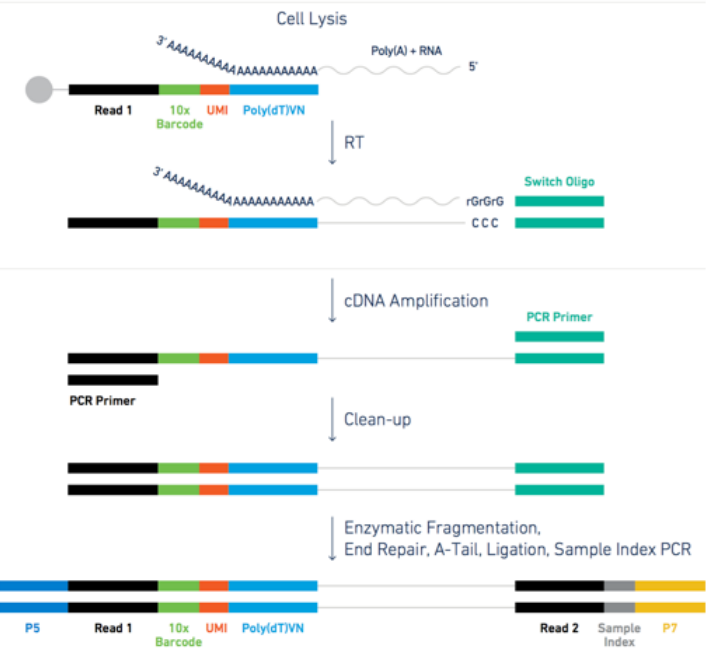
\includegraphics[width=6.25in,height=\textheight]{images/10X.png}

}

\caption{\label{fig-steps}steps for the microdroplet-based single cell
RNA sequencing after isolation.}

\end{figure}%

\subsection{The raw data in practice}\label{the-raw-data-in-practice}

Let's look at a specific read and its UMI and cell barcode. The data is
organized in paired-end reads (written on \texttt{fastq} files), where
the first \texttt{fastq} file contains reads in the following format

\begin{verbatim}
@SRR8363305.1 1 length=26
NTGAAGTGTTAAGACAAGCGTGAACT
+SRR8363305.1 1 length=26
#AAFFJJJJJJJJJJJJJJJJFJJJJ
\end{verbatim}

Here, the first 16 characters \texttt{NTGAAGTGTTAAGACA} represent the
cell barcode, while the last 10 characters \texttt{AGCGTGAACT} are the
transcript UMI tag. The last line represents the quality scores of the
26 characters of barcode+UMI.

The associated second \texttt{fastq} file contains reads of 98nt as the
following

\begin{verbatim}
@SRR8363305.1 1 length=98
NCTAAAGATCACACTAAGGCAACTCATGGAGGGGTCTTCAAAGA
    CCTTGCAAGAAGTACTAACTATGGAGTATCGGCTAAGTCAANCN
    TGTATGAGAT
+SRR8363305.1 1 length=98
#A<77AFJJFAAAJJJ7-7-<7FJ-7----<77--7FAAA--
    <JFFF-7--7<<-F77---FF---7-7A-777777A-<
    -7---#-#A-7-7--7--
\end{verbatim}

The 98nt-long string of characters in the second line is a partial
sequence of the cDNA transcript. Specifically, the 10X chromium protocol
used for sequencing the data is biased towards the 3' end, because the
sequencing is oriented from the 3' to the 5' end of the transcripts. The
last line contains the corresponding quality scores.

\subsection{Alignment and expression
matrix}\label{alignment-and-expression-matrix}

We aligned the data with \texttt{cellranger}, a completely automatized
\href{https://support.10xgenomics.com/single-cell-gene-expression/software/pipelines/latest/what-is-cell-ranger}{pipeline
implemented by 10X} for 10X-genomics data.

Apart from the data, the output contains an interactive document
(\texttt{web\_report.html}) reporting the quality of the data and a
small preliminary UMAP plot and clustering . In this report it is
especially instructive to look at the \textbf{knee plot}.

The knee plot is created by plotting the number of unique molecular
identifiers (UMIs) or reads against the number of cells sequenced,
sorted in descending order. The UMIs or reads are a measure of the
amount of RNA captured for each cell, and thus a measure of the quality
of the data. The plot typically shows a \textbf{steep slope at the
beginning, followed by a plateau, and then a gradual decrese into a
second slope and a final plateau}.

\begin{itemize}
\tightlist
\item
  The steep slope represents the initial cells that are of \textbf{high
  quality} and have the highest number of UMIs or reads.
\item
  The first plateau represents the cells that have \textbf{lower quality
  data}, and the gradual decrease represents the addition of droplets
  with even lower quality data.
\item
  Usually, beyond the first slope, you have droplets that are
  \textbf{either empty or of so poor quality}, that they are not worth
  keeping for analysis.
\item
  The height of the last plateau gives you an idea of the
  \textbf{presence of ambient RNA} inside droplets. If the last plateau
  is located high up, then the corresponding amount of UMIs consist of
  background ambient RNA which likely pollutes all cells in your data.
\end{itemize}

Below, the knee plot from the \texttt{control\ 1} sample used in this
course's analysis tutorial. You can see that around 10,000 cells with
above \textasciitilde1000 UMIs seems to be coinsidered of decent quality
by \texttt{cellranger} (the part of line coloured in blue). Note that
the last plateau is located at a very low amount of UMIs, meaning there
is not really any relevant contamination from ambient RNA.

\begin{figure}

\centering{

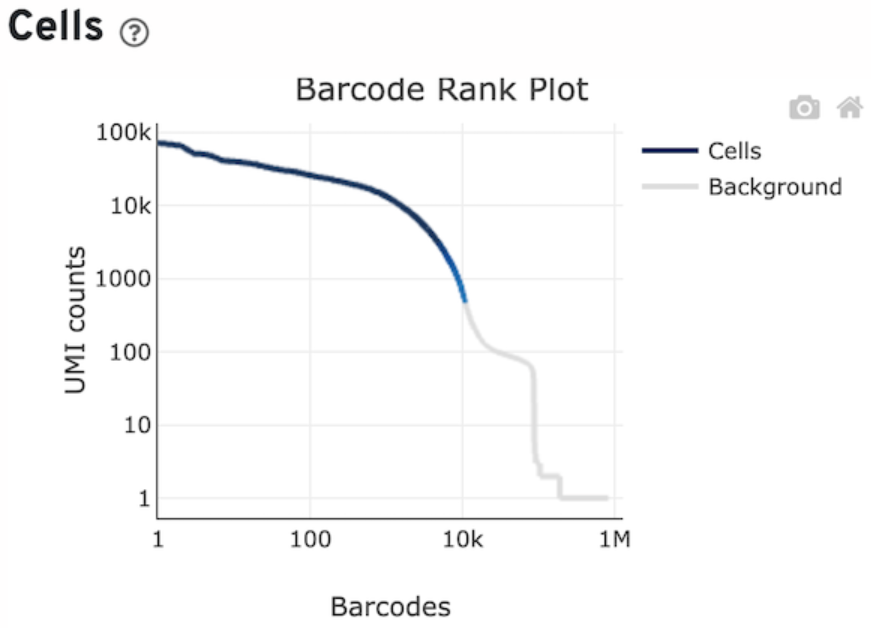
\includegraphics[width=6.25in,height=\textheight]{images/knee.png}

}

\caption{\label{fig-knee}Knee plot of the Control 1 sample of the
tutorial. Note the lower plateau of ambient RNA}

\end{figure}%

\begin{tcolorbox}[enhanced jigsaw, colbacktitle=quarto-callout-note-color!10!white, left=2mm, breakable, bottomtitle=1mm, colframe=quarto-callout-note-color-frame, opacityback=0, opacitybacktitle=0.6, toprule=.15mm, colback=white, toptitle=1mm, titlerule=0mm, arc=.35mm, title={Exercise}, bottomrule=.15mm, rightrule=.15mm, leftrule=.75mm, coltitle=black]

In the folder \texttt{Alignment\_results} you have the document
\texttt{web\_summary.html} that shows you the quality report of your
small toy dataset. \textbf{Take some time to look at it and explore what
it contains} (Click on \texttt{Trust\ HTML} on the top menu if the html
remains blank after opening it).

\end{tcolorbox}

The background RNA (sequenced together with the transcript coming from
the cell of interest) makes up the \emph{ambient plateau}: the same
background RNA is contained in empty droplets. If your dataset has
extremely few UMI counts in empty droplets, then there is not much
background RNA present - This is the best situation in which you can
find yourself. See Exhibit A in Figure~\ref{fig-bender}.

If you have a dataset where you can identify an \emph{empty droplet
plateau} by eye (Exhibit B in Figure~\ref{fig-bender}), and these empty
droplets have 50 or 100 or several hundred counts, then it can be
advisable to use a specific software to remove the background
transcripts (e.g.~\texttt{CellBender} (Fleming et al. (2023)),
\texttt{SoupX} (Young and Behjati (2020))).

If you have a dataset with so much background RNA that you cannot
identify the \emph{empty droplet plateau} yourself by eye (Exhibit C in
Figure~\ref{fig-bender}), then any software to remove background
transcripts will also likely have a difficult time. Such the algorithms
might be worth a try, but you should \textbf{strongly consider
re-running the experiment, as the knee plot points to a real QC failure}

\begin{figure}

\centering{

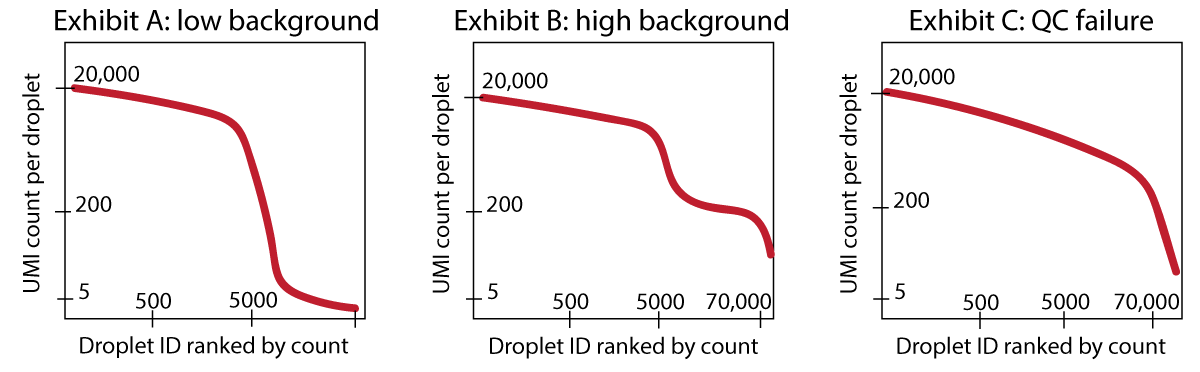
\includegraphics[width=6.25in,height=\textheight]{images/UMI_curve_tropes.png}

}

\caption{\label{fig-bender}Various cases of knee plot you can encounter
from sequenced data. Figure from
\href{https://cellbender.readthedocs.io/}{the webpage of Cellbender.}}

\end{figure}%

\subsection{What does SoupX do}\label{what-does-soupx-do}

Before we get started with the specifics of example data sets and using
the R package, it is worth understanding at a broad level what the
problem this package aims to solve is and how it goes about doing it.

In droplet based, single cell RNA-seq experiments, there is always a
certain amount of background mRNAs present in the dilution that gets
distributed into the droplets with cells and sequenced along with th
(see Figure~\ref{fig-bender} again)em The net effect of this is to
produce a background contamination that represents expression not from
the cell contained within a droplet, but the solution that contained the
cells.

This collection of cell free mRNAs floating in the input solution
(henceforth referred to as ``the soup'') is created from cells in the
input solution being lysed. Because of this, the soup looks different
for each input solution and strongly resembles the expression pattern
obtained by summing all the individual cells.

The aim of this package is to provide a way to estimate the composition
of this soup, what fraction of UMIs are derived from the soup in each
droplet and produce a corrected count table with the soup based
expression reoved.

The method to do this consists of three parts:

\begin{enumerate}
\def\labelenumi{\arabic{enumi}.}
\tightlist
\item
  Calculate the profile of the soup.
\item
  Estimate the cell specific contamination fraction.
\item
  Infer a corrected expression matrix.
\end{enumerate}

In previous versions of SoupX, the estimation of the contamination
fraction (step 2) was the part that caused the most difficulty for the
user. The contamination fraction is parametrised as \texttt{rho} in the
code, with \texttt{rho=0} meaning no contamination and \texttt{rho=1}
meaning 100\% of UMIs in a dropeNowon 1.3.0 onwards, an automated
routine for estimating the contamination fraction is provided, which
should be suitable is mostw it can fail.

While it is possible to run SoupX without clustering information, you
will get far better results if some basic clustering is provided.
Therefore, it is \textbf{strongly} recommended that you provide some
clustering information to SoupX. If you are using 10X data mapp (as in
our case)ed with cellranger, the default clustering produced by
cellranger is automatically loaded and used. The results are not
strongly sensitive to thed similar results.

\section{Loading SoupX}\label{loading-soupx}

We start by loading the necessary soupX package necessary for the
analysis

\begin{Shaded}
\begin{Highlighting}[]
\FunctionTok{library}\NormalTok{(SoupX)}
\end{Highlighting}
\end{Shaded}

Here \texttt{SoupX} performs the three main steps to decontaminate data.
We only need to provide the alignment output, and the rest is
automatical. You can find a more complex tutorial with all perks of
\texttt{SoupX}
\href{https://github.com/constantAmateur/SoupX/blob/master/vignettes/pbmcTutorial.Rmd}{here}

\begin{Shaded}
\begin{Highlighting}[]
\NormalTok{sc }\OtherTok{=} \FunctionTok{load10X}\NormalTok{(}\StringTok{\textquotesingle{}./aligned\_data/outs/\textquotesingle{}}\NormalTok{)}
\NormalTok{sc }\OtherTok{=} \FunctionTok{autoEstCont}\NormalTok{(sc)}
\NormalTok{out }\OtherTok{=} \FunctionTok{adjustCounts}\NormalTok{(sc)}
\end{Highlighting}
\end{Shaded}

\begin{verbatim}
Loading raw count data

Loading cell-only count data

Loading extra analysis data where available

216 genes passed tf-idf cut-off and 194 soup quantile filter.  Taking the top 100.

Using 714 independent estimates of rho.

Estimated global rho of 0.04

Warning message in sparseMatrix(i = out@i[w] + 1, j = out@j[w] + 1, x = out@x[w], :
“'giveCsparse' is deprecated; setting repr="T" for you”
Expanding counts from 15 clusters to 4931 cells.
\end{verbatim}

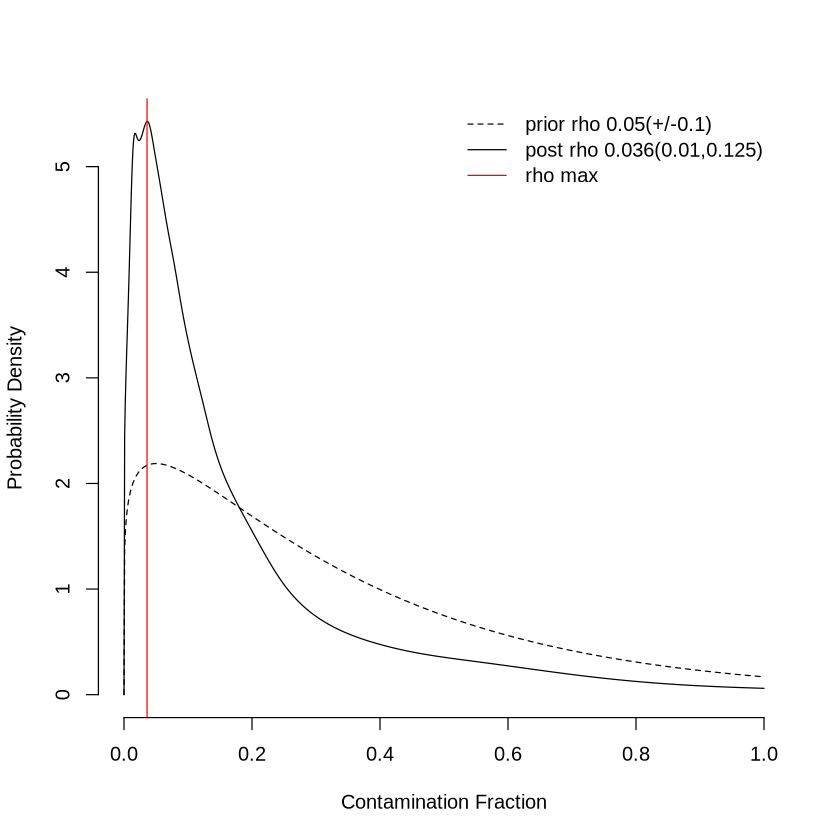
\includegraphics{Cleaningthedata.source_files/figure-pdf/cell-3-output-2.png}

You should get an output showing - with a solid line - a distribution of
the contamination of each gene. In our toy dataset, the contamination is
pretty low, as it could be seen from the knee plot in the web report.

You can also use the tSNE plot of a specific gene to reveal how many
transcripts have been changed due to contamination.

\begin{Shaded}
\begin{Highlighting}[]
\FunctionTok{plotChangeMap}\NormalTok{(sc,out,}\StringTok{\textquotesingle{}LotjaGi2g1v0360900\textquotesingle{}}\NormalTok{)}
\end{Highlighting}
\end{Shaded}

\begin{tcolorbox}[enhanced jigsaw, colbacktitle=quarto-callout-note-color!10!white, left=2mm, breakable, bottomtitle=1mm, colframe=quarto-callout-note-color-frame, opacityback=0, opacitybacktitle=0.6, toprule=.15mm, colback=white, toptitle=1mm, titlerule=0mm, arc=.35mm, title=\textcolor{quarto-callout-note-color}{\faInfo}\hspace{0.5em}{Wrapping Up}, bottomrule=.15mm, rightrule=.15mm, leftrule=.75mm, coltitle=black]

This is the end of the tutorial - it was mostly ment to let you get
confidence with a jupyter notebook and the data decontamination process.
We will use decontamination also on the real dataset.

\end{tcolorbox}

\phantomsection\label{refs}
\begin{CSLReferences}{1}{0}
\bibitem[\citeproctext]{ref-fleming_unsupervised_2023}
Fleming, Stephen J., Mark D. Chaffin, Alessandro Arduini, Amer-Denis
Akkad, Eric Banks, John C. Marioni, Anthony A. Philippakis, Patrick T.
Ellinor, and Mehrtash Babadi. 2023. {``Unsupervised Removal of
Systematic Background Noise from Droplet-Based Single-Cell Experiments
Using {CellBender}.''} \emph{Nature Methods} 20 (9): 1323--35.
\url{https://doi.org/10.1038/s41592-023-01943-7}.

\bibitem[\citeproctext]{ref-young_soupx_2020}
Young, Matthew D, and Sam Behjati. 2020. {``{SoupX} Removes Ambient
{RNA} Contamination from Droplet-Based Single-Cell {RNA} Sequencing
Data.''} \emph{GigaScience} 9 (12): giaa151.
\url{https://doi.org/10.1093/gigascience/giaa151}.

\end{CSLReferences}



\end{document}
